% !TEX root=../master.tex

\chapter{Experimental Apparatus}
\label{chp:experimental_apparatus}

This chapter describes the software and hardware used in the experiments that
are detailed in Chapters~\ref{chp:estimation_paper} and~\ref{chp:control_paper}.

\section{Software}
\subsection {ROS}
The same C++ algorithm implementations are used both in hardware and simulation
experiments.
This is made possible, in part, due to the use of the Robot Operating System\footnote{Robot Operating System:
\href{www.ros.org}{www.ros.org}} (ROS) as a middleware. ROS provides a way for separate
programs, or nodes, to share information between one another.

A network diagram of the software system can be seen in~\figref{fig:network_diagram}. The estimator and
controller for the UAV are implemented as two separate nodes, where the
estimator node provides the state estimate of the UAV to the controller node.
The controller node computes the desired control action based on the error
between the estimated state and the desired state. This desired control action
is sent to the ROSflight flight control stack~\cite{jackson2016rosflight}
which then actuates either a simulated UAV or the real hardware platform.

\begin{figure}[htbp]
  \centering
  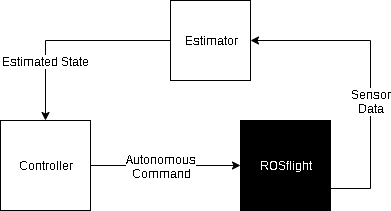
\includegraphics[width=3.5in]{figures/roscopter.png}
  \caption[Software Architecture Network Diagram]{A network diagram of the
  software running during both simulation and hardware experiments.}
%
  \label{fig:network_diagram}
\end{figure}

\subsection {Gazebo}
For simulation experiments, the Gazebo\footnote{Gazebo:
\href{www.gazebosim.org}{www.gazebosim.org}} simulation environment was used with the ROSflight software-in-the-loop
(SIL) simulation. This simulation setup allows the
same estimator and controller implementations to
be used in the simulation experiments as are used in the hardware experiments,
making the transition from simulation to hardware less difficult.

\subsection {ROScopter}
The estimator and controller nodes of the ROScopter\footnote{ROScopter:
\href{www.github.com/byu-magicc/roscopter}{www.github.com/byu-magicc/roscopter}}
project were also used at certain points during the simulation and hardware
experiements described in this thesis. In the experiments of the estimator proposed in
Chapter~\ref{chp:estimation_paper}, the ROScopter controller node was used to
close the loop around the estimates produced. In the experiments of the 
controller proposed in Chapter~\ref{chp:control_paper}, the ROScopter estimator node
was used to provide state estimates of the UAV to the controller.

\section{Hardware}
The multirotor UAV used in hardware experiments can be seen
in~\figref{f:drone_pic}. The UAV is built on a DJI Flamewheel 450 frame.
Specific components contained on the UAV are detailed in the following
subsections.

\subsection{Flight Controller}
The multirotor UAV is equipped with an OpenPilot CC3D Revolution 32 bit F4
flight controller as shown in~\figref{fig:f4}. The flight controller runs the
ROSflight firmware which provides an easy interface
for the controller running on the onboard computer to control the UAV.

\begin{figure}[htbp]
  \centering
  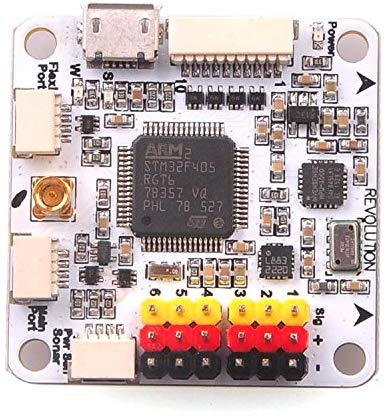
\includegraphics[width=2.5in]{figures/f4.jpg}
  \caption[OpenPilot CC3D Revolution 32 bit F4]{\MF{Cite these images?} The OpenPilot CC3D Revolution 32
  bit F4 flight controller used in experiments.}
%
  \label{fig:f4}
\end{figure}

\subsection{Onboard Computer}
The computer onboard the UAV is an NVIDIA Jetson TX2 equipped with an Orbitty
Carrier board. This configuration is shown in~\figref{fig:tx2_orbitty}. All
computation was done on the onboard computer during the hardware experiments.

\begin{figure}[h]
  \centering
  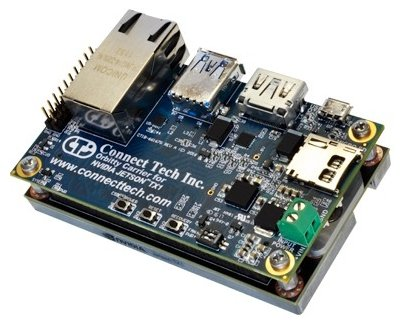
\includegraphics[width=2.5in]{figures/tx2_orbitty.jpg}
  \caption[NVIDIA Jetson TX2 with Orbitty Carrier Board]{The NVIDIA Jetson TX2
  with an Orbitty carrier board attached.
  % This is the configuration of the
% onboard computer used in the flight experiments described in this thesis.}
  }
%
  \label{fig:tx2_orbitty}
\end{figure}

\subsection{Motion Capture}
Hardware flight experiments were performed in the motion capture room in the
MAGICC Lab at Brigham Young University. This room is equipped with an OptiTrack\footnote{OptiTrack:
\href{www.optitrack.com}{www.optitrack.com}} motion tracking system that
provides high-rate measurements of the position and attitude of the multirotor
UAV during flight.

\subsection{Camera}
For the hardware experiments described in Chapter~\ref{chp:estimation_paper},
the multirotor UAV was outfitted with an ELP USB camera with a 2.1 mm lens as
shown in~\figref{fig:camera}. The intrinsic parameters of the sensor were
accurately calibrated using a software package provided by ROS\footnote{ROS
camera\_calibration: \href{wiki.ros.org/camera_calibration}{wiki.ros.org/camera\_calibration}},
however, the mounting position and attitude of the camera were only roughly
approximated.

\begin{figure}[h]
  \centering
  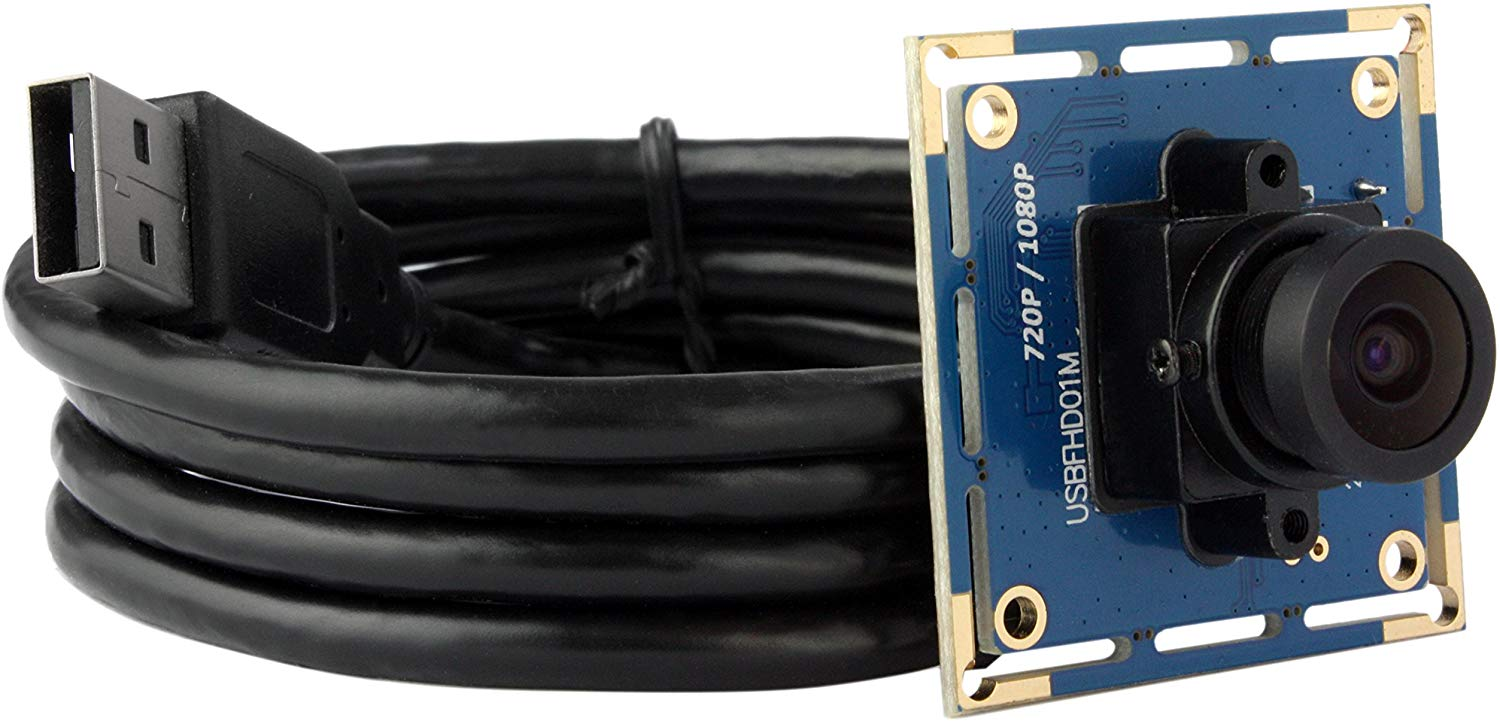
\includegraphics[width=2.5in]{figures/camera.jpg}
  \caption[ELP USB Camera with 2.1 $mm$ Lens]{An ELP USB Camera with a 2.1 mm
  lens as used on the multirotor UAV during flight experiments.}
%
  \label{fig:camera}
\end{figure}

